% !TEX root = ../thesis.tex
\chapter{Introduction}
\label{chap:Intro}
\label{sec:intro}

\begin{comment}
\begin{figure}%[h]
\centering
% left bottom right top
\includegraphics[clip= true, width= \columnwidth, trim= 0in 0.0in 0.0in 1.3in]{pictures/architecture.pdf}
\caption{Architecture.}
\label{fig:architecture}
\end{figure}
\end{comment}
%

The way network services are delivered has dramatically changed in the last few years thanks to the arise of the Network Functions Virtualization (NFV) paradigm, which allows network services to experiment the same degree of flexibility and agility already available in the cloud computing world.
In fact, NFV proposes to transform the network functions that today run on dedicated appliances (e.g., firewall, WAN accelerator) into a set of software images that can be consolidated into high-volume standard servers, hence replacing those middleboxes with the so called Virtual Network Functions (VNFs).

NFV is currently being seen as a technology targeting network operators, which can exploit the power of the IT virtualization (e.g., cloud and datacenters) to deliver network services with unprecedented agility and efficiency.
However, end users have never been taken into consideration as active players in the NFV domain; furthermore, NFV is limited to the datacenter, leaving most of the telecom operator network out of the picture. 

This thesis tries to invert this trend by presenting a solution that is oriented to deliver \textit{generic} network services, selected by \textit{multiple actors}, which allows
the \textit{dynamic} instantiation of \textit{per-user} network services.
In future, this can be used on the large infrastructure of the telecom operators, possibly starting from the home gateway installed in the customer premises till the data center, as depicted in Figure~\ref{fig:ISPnetwork}.


Our solution enables several actors (e.g., network providers, end users such as the xDSL customers, etc.) to define their preferred network services; moreover, is it general enough 
%Our model is general enough 
that services include both the traditional middlebox functions considered in NFV as well as traditional host-based network services.
For example, the network service selected by a customer can include a deep packet inspection (DPI) VNF that handles HTTP traffic, an email scanner to analyze and clean his electronic correspondence, and a Bittorrent client that downloads the objects specified by the user without interfering with the rest of the traffic.
In our solution, the entire network infrastructure is controlled by a service logic that performs the identification of the user that is connecting to the network itself.
Upon a successful identification, the proper set of network functions chosen by the user is instantiated in one of the nodes (possibly, even the home gateway) available on the provider network, and the physical infrastructure is configured to deliver the user traffic to the above set of VNFs.

\begin{figure}%[h]
	\centering
	% left bottom right top
	\includegraphics[clip= true, width= 0.7\columnwidth, trim= 0in 0.5in 0.0in 0.5in, page= 33]{images/Pictures_definitivo.pdf}
	\caption{Deployment of virtual network functions on the wide telecom provider network.}
	\label{fig:ISPnetwork}
\end{figure}

More in detail, the thesis describes the service-oriented layered architecture to achieve those objectives, a possible set of data models that are used to describe and implement the requested network services (starting from an high-level and user-friendly view of the service, which is then converted into a set of primitives (e.g., virtual machines, virtual links) that are actually used to instantiate the service on the physical infrastructure), and two possible implementations of the nodes of the infrastructure layer on which the service is actually deployed.

Particularly, we explored two solutions for the nodes hosting the VNFs, which are based on different technologies and have different requirements in terms of hardware resources.
The first proposal is based on the OpenStack open-source framework, and it is more appropriate to be integrated in (existing) cloud environments; the second one, instead, exploits mostly dedicated software, and it is oriented either to demanding environments (e.g., high performance network services) or to the embedded segment (resource-constrained CPE). This second infrastructure layer have been implemented by other netgroup members and is presented in this thesis only for validate the higher layers of the architecture. 

The reminder of this thesis is structured as follows. 
Chapter~\ref{chap:Problem} details the reasons that led us to adopt an NFV and SDN approach in our architecture.
Chapter~\ref{chap:State of the Art} provides an overview of the related works, in particular the ETSI NFV, while Chapter~\ref{chap:Utilized Tools} gives a detailed overview of OpenStack  and OpenDaylight (an open-source SDN controller), which are used in our architecture. Chapter~\ref{sec:gen_arch} introduces an architecture to deploy general network services on the wide provider network, while Chapter~\ref{sec:data_model} details some formalisms expressing the service to be deployed, which are then exploited in the use case discussed in the first section of Chapter~\ref{sec:implementation}.
Chapter~\ref{sec:implementation} details the preliminary implementation of the architecture, which is then validated in Chapter~\ref{sec:validation}, both in terms of functionalities and performance.
Finally, Chapter~\ref{sec:conclusion} concludes the thesis and provides some plans for the future.